\documentclass[11pt,a5paper]{article}
\usepackage{xcolor}
\usepackage[T1]{fontenc}
\usepackage[utf8]{inputenc}
\usepackage[italian]{babel}
\usepackage{alltt}
\usepackage{scrextend}
\usepackage{geometry}
\usepackage[default]{opensans}
\usepackage{eso-pic}
\usepackage{tikz}
\usepackage{titlesec}
\usepackage[most]{tcolorbox}
\definecolor{block-gray}{gray}{0.82}
\newtcolorbox{myquote}{colback=block-gray,grow to right by=-10mm,grow to left by=-10mm, boxrule=0pt,boxsep=0pt,breakable}

\usepackage{graphicx}
\usepackage{transparent}
\usepackage{ifthen}

\newif\iflogo

\AddToShipoutPictureBG{
  \iflogo{%
    \put(280,390){%
      \transparent{0.17}
\includegraphics[width=3.5cm]{logo_SNS_nero}%
    }%
  }\else\fi%
}

\makeatletter
\renewcommand{\@seccntformat}[1]{%
  \begingroup
  \@nameuse{additional@cntformat#1}%
  {\@nameuse{the#1}}%
  \endgroup
  \quad
}
\newcommand{\setformat}[2]{%
  \@namedef{additional@cntformat#1}{#2}%
}
\makeatother

\setformat{section}{\LARGE}

\newcommand{\santanna}{{\normalsize s}ant'{\normalsize a}nna}
\newcommand{\subtitle}[1]{\vspace*{-0.8em}{\hskip 1.0cm\textcolor{gray}{\fontsize{11.5}{16}\selectfont\it #1}}\vspace*{0em}}
\let\oldsection\section
\renewcommand{\section}[1]{%
  \vskip 1.0cm plus 1.0cm minus 0.5cm%
  \oldsection{\fontfamily{ppl}\selectfont\fontsize{16}{24}\selectfont\scshape{#1}}%
  \vspace*{-0.6em}%
}
\renewcommand{\title}[1]{%
  \vspace*{-2em}%
  {\fontfamily{pag}\selectfont\scshape\Huge{#1}}%
  \vspace*{2em}%
}

\newenvironment{canzone}{%
  \begin{addmargin}[1cm]{0cm}%
  \begin{alltt}\normalfont%
  }{%
  \end{alltt}%
  \end{addmargin}%
}

\begin{document}
\logofalse
\newgeometry{top=0mm,bottom=0mm,left=0mm,right=0mm}
\fontsize{13}{16}\selectfont
\setlength{\parindent}{0cm}
\setlength{\parskip}{1em plus 0.2em minus 0.2em}
\linespread{1.25}
\pagestyle{empty}

%% -- PRIMA DI COPERTINA
\leavevmode
\put(50,90){
  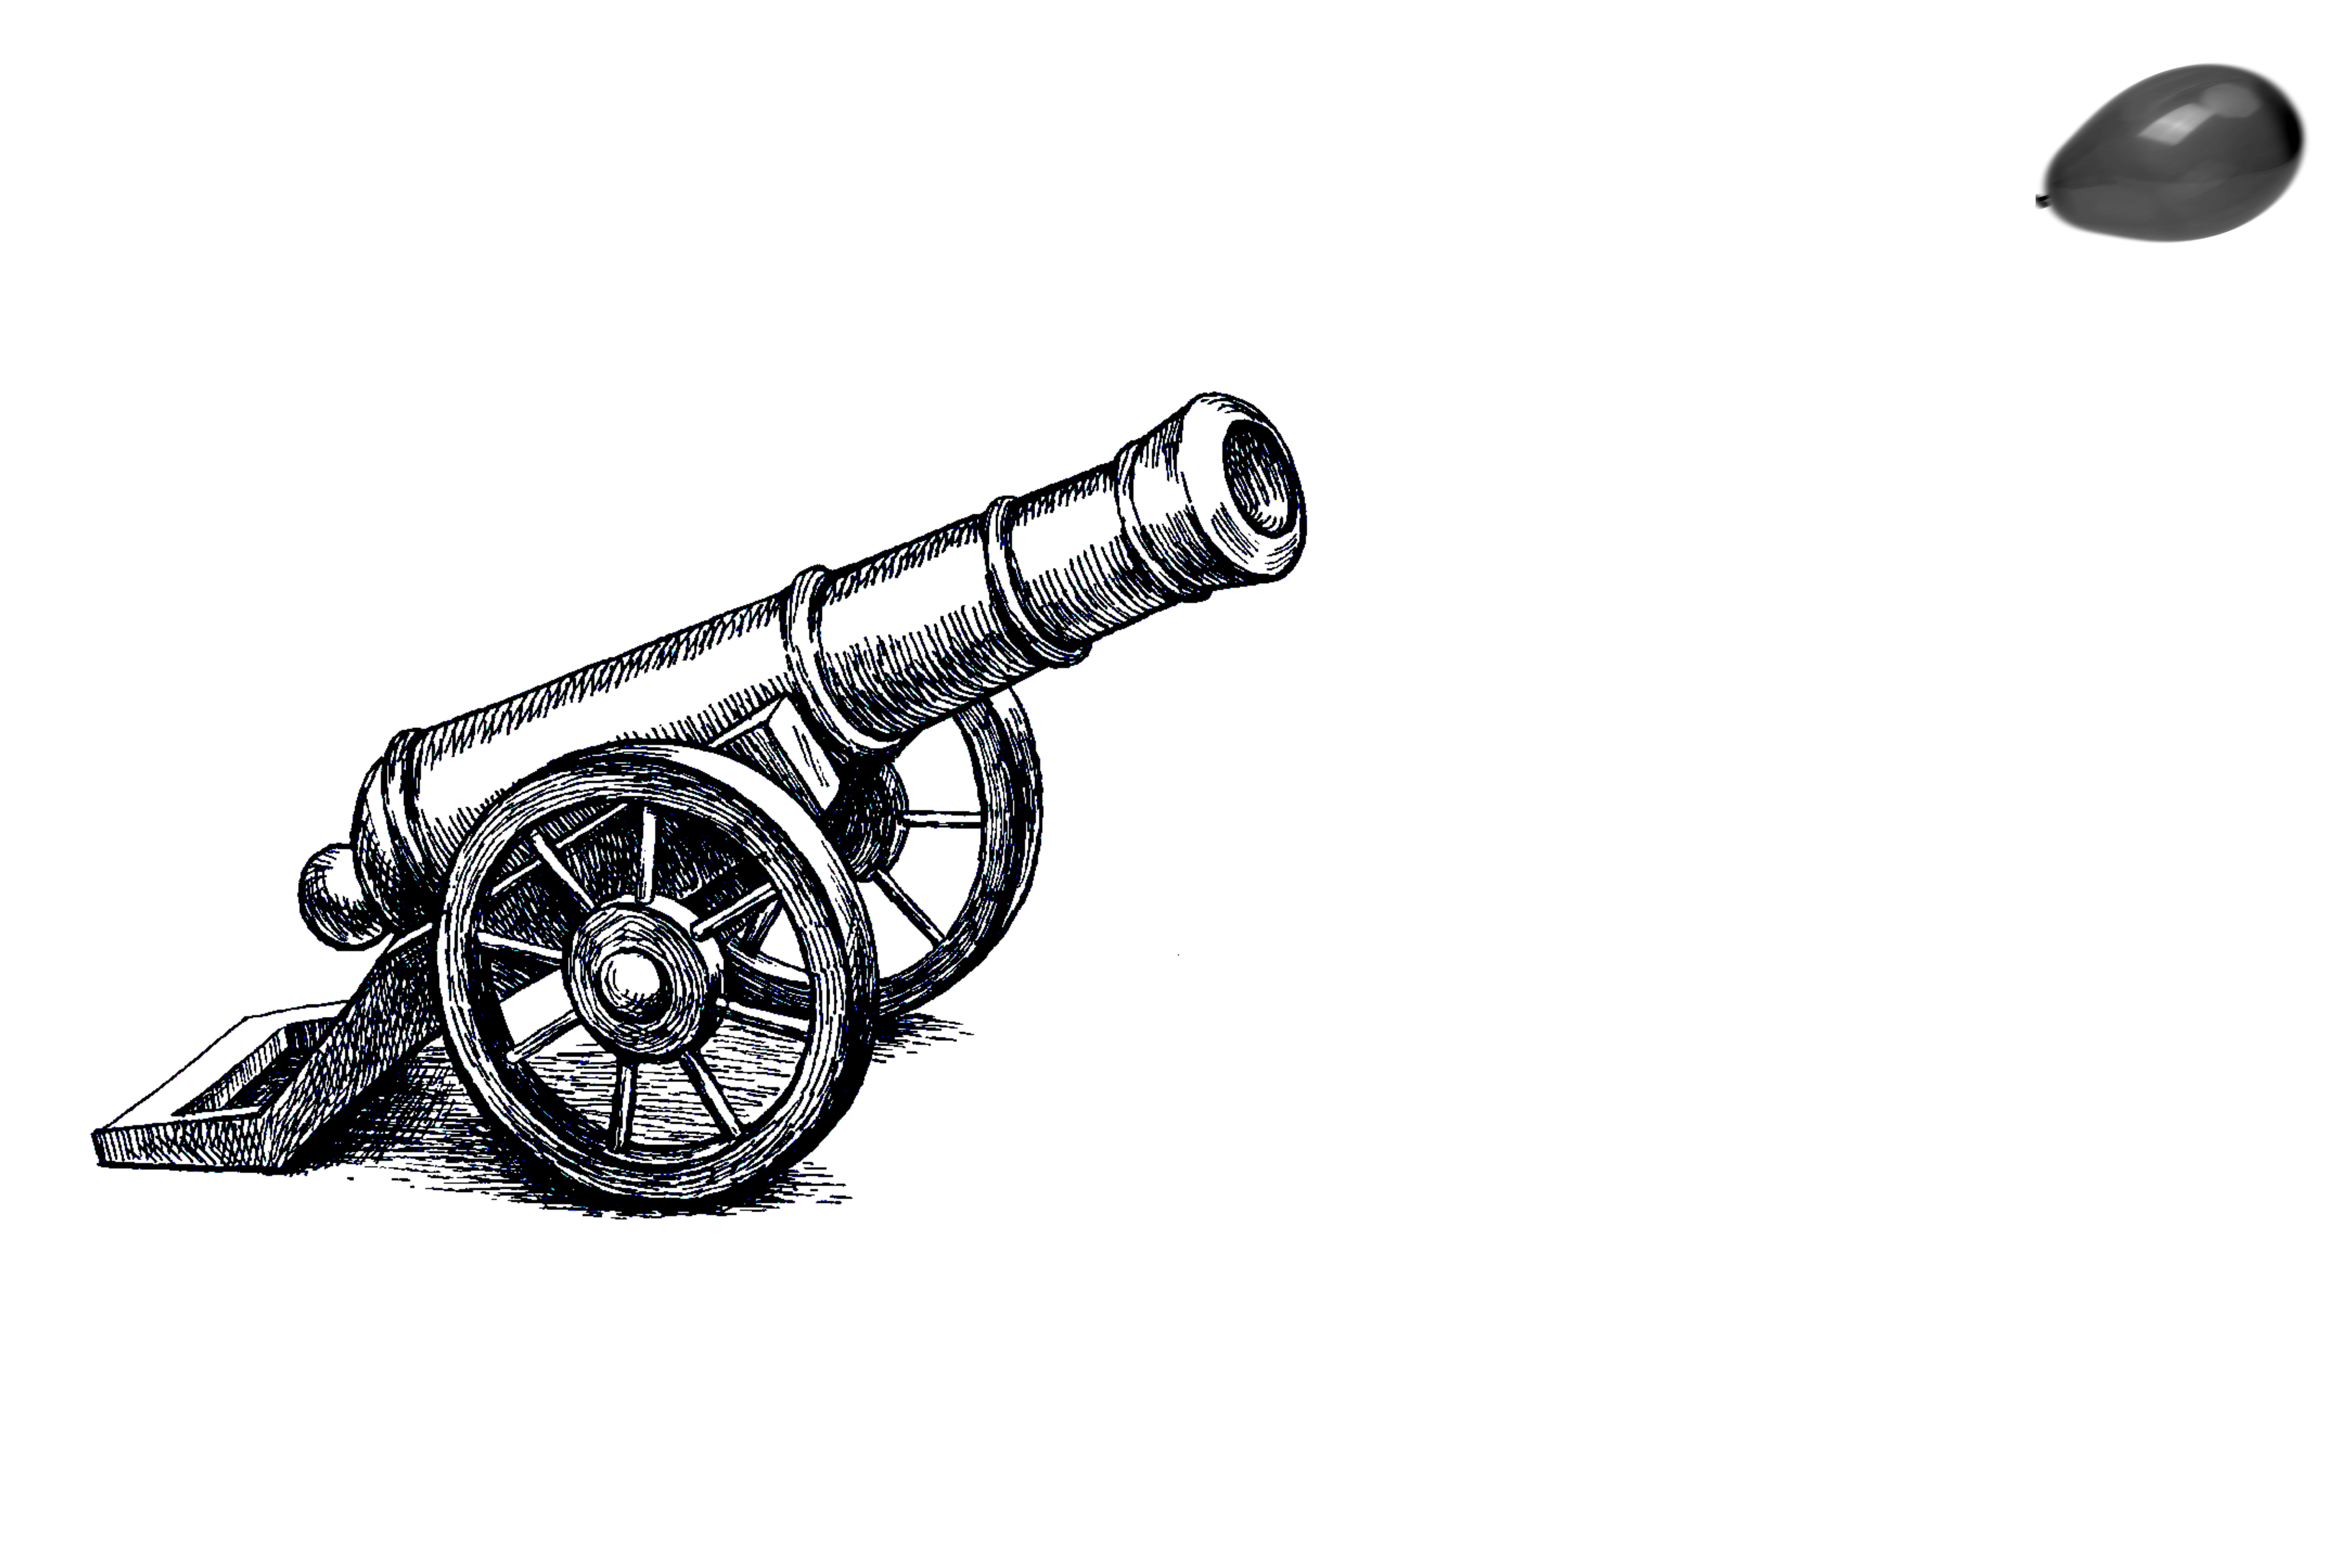
\includegraphics[width=0.70\textwidth]{miniatura}
}
\leavevmode
\put(0,0){
  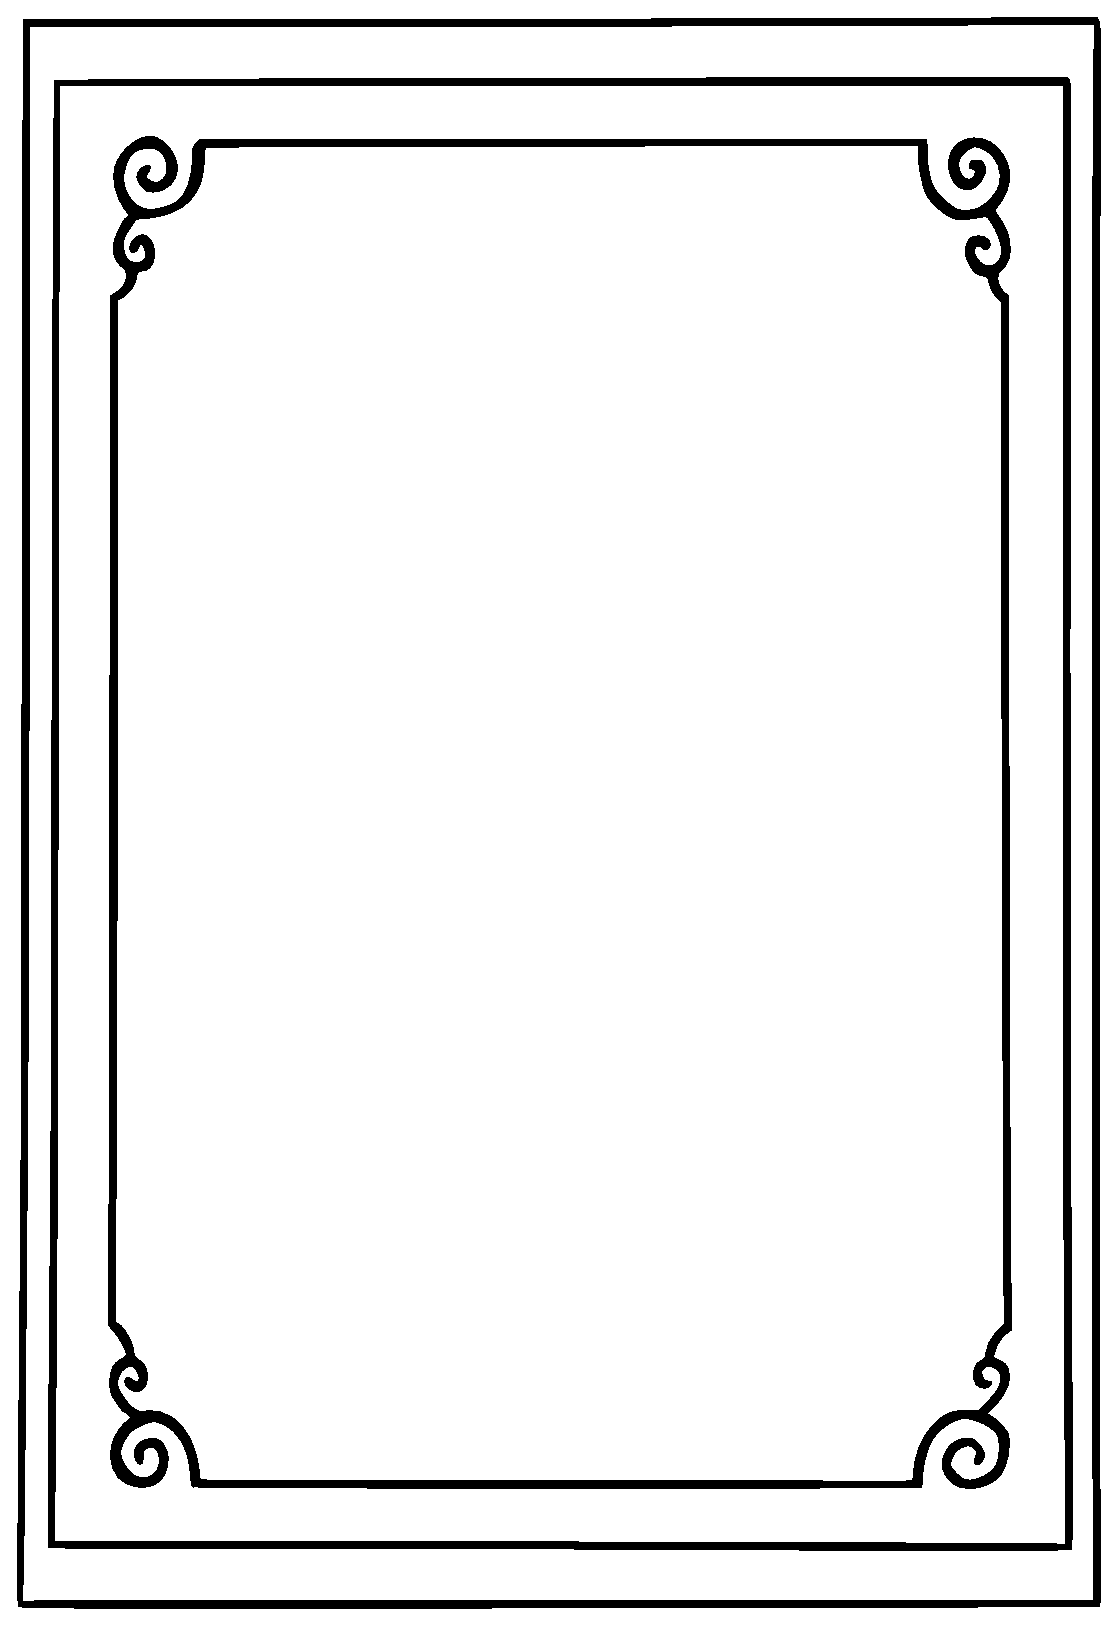
\includegraphics[width=0.96\textwidth]{cornice}
}
\leavevmode
\put(60,300){
  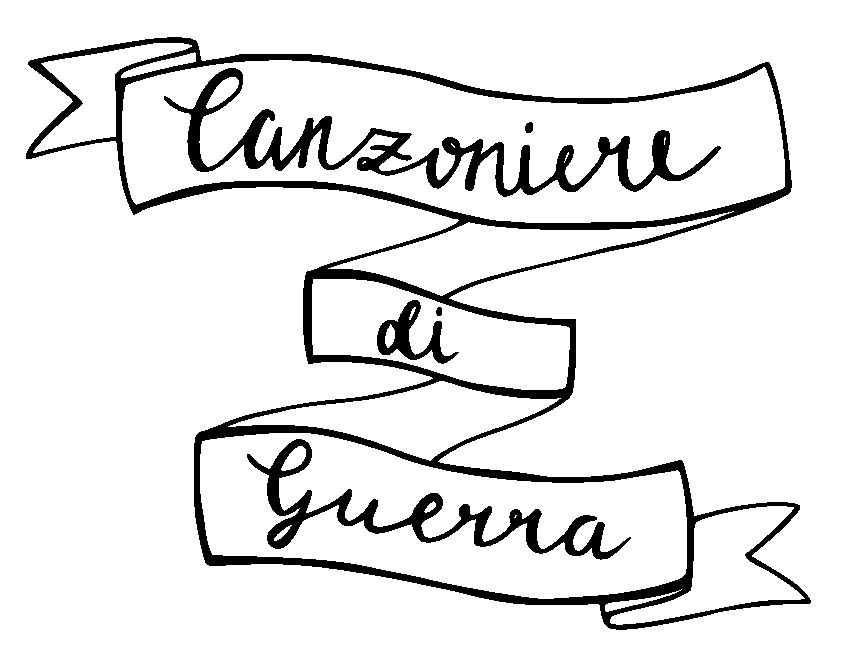
\includegraphics[width=0.70\textwidth]{striscione}
}
\leavevmode
\put(265,60){
  {\transparent{0.8}
\includegraphics[width=0.16\textwidth]{fregio}}
}
\clearpage
\newgeometry{top=17mm,left=15mm,right=15mm,bottom=20mm}
%% -- CITAZIONE E RINGRAZIAMENTI
\begin{myquote}\it
  Chi vince la guerra scrive la storia,\\
  chi perde la guerra scrive i giornali.
  
  {~\hfill\normalfont -- Gianni Cusumano}
\end{myquote}

\vfill

\begin{minipage}{0.80\textwidth}\fontsize{10}{15}\selectfont
  Cornice e Titolo di Marta Tasinato \\
  Adeguamento Immagini di Piero Lafiosca ed Enrico Polesel \\
  Correzione testi di ... \\
  Impaginazione e Layout di Dario Balboni
\end{minipage}
\clearpage
\logotrue
%% -- INIZIO DEL CANZONIERE
\title{Canzoniere di Guerra}

\section{Scuola Normale trionferà}
\subtitle{cantata sul tema di “Bandiera Rossa”}
\begin{canzone}
Puzza di fogna, ti attacca il tifo,
pidocchi e rogna, fa proprio schifo.
È il santannino, è un animale,
ma la Normale lo domerà.

Scuola Normale la trionferà,
Scuola Normale la trionferà,
e il santannino che la sfiderà
lavato con Perlana si ritirerà.

Noi integriamo gli operatori,
campi finiti, quadritensori...
mentre al sant'Anna che gran buffoni,
solo addizioni sapete far!

Scuola Normale la trionferà,
Scuola Normale la trionferà,
e il santannino che la sfiderà
lavato con Perlana si ritirerà.

I santannini sono ingegneri,
sono giuristi, son parrucchieri.
Ma quale genio? Ma che eccellenza?
La vera scienza si fa in Normal!

Scuola Normale la trionferà,
Scuola Normale la trionferà,
Scuola Normale la trionferà,
Se liberiam Barbieri chi vi salverà?
Se liberiam Barbieri chi ci salverà?
\end{canzone}

\section{Alla Normale urrà}
\subtitle{cantata sul tema di “When Jhonny comes marching home”}
\begin{canzone}
È pronta la Normale per le avversità,
abbiam giurato tutti non aver pietà:
i gavettoni alla fanteria,
dalle finestre l'artiglieria,
fremono gli idranti.
Per la Normale urrà!

Non hanno i santannini alcuna dignità,
son tutti dei fascisti figli di papà,
non han fatto neanche un bidet
sin dal lontano sessantatré:
è arrivato il puzzo
sino in Normale già.

Vedendoli fuggire ed implorar pietà
mostriamo ai loro anziani cos'è l'umiltà
e da sevizie ridicole
salviam le loro matricole
che dovran la vita
alla Normale urrà! 
\end{canzone}

\section{Son perdenti, son sfigati}
\subtitle{sulla canzoncina tipica dei marines}
\begin{canzone}
Son perdenti, son sfigati,
i giuristi e gli avvocati!
Gli ingegneri che buffoni,
sbaglian pure le addizioni!

Destinato è il santannino,
solo a fare lo spazzino!
Canta in cor la nostra truppa,
S.S.S.U.Puppa!
\end{canzone}

\section{Il ponte sul Fiume Arno}
\begin{canzone}
Guarda, che cosa vedi là?
Sembra il culo d'un maial.
E invece, è un santannino,
Steccò persino il test in Normal!

Puzza, come un animal,
Studia, ma resta un gran somar,
Merda, di un santannino,
Fatti vicino, ti devo lavar!
\end{canzone}

\section{\santanna\ Merda}
\begin{canzone}
Sant'Anna merda, Sant'Anna colera
Sei la rovina dell'Italia intera.

O' santannino, lavora duro
Che alla Normale devi dare pure il culo.

Santannino figlio di puttana,
Santannino figlio di puttana (ad libitum)
\end{canzone}

\section{Normale Olè}
\begin{canzone}
Normale olè, Normale olè,
Forza Normale, Normale olè!
Normale olè, Normale olè,
Forza Normale, ...Normale olè!

Se le scuole sono tante,
la migliore resti tu,
sei l'orgoglio del Priore,
che ci guida da lassù,

E la feccia santannina,
fu la nostra succursal,
ora trema poverina,
se ci sente cantar:

Normale olè, Normale olè,
Forza Normale, Normale olè!
Normale olè, Normale olè,
Forza Normale, ...Normale olè!
\end{canzone}

\section{Sono gli Scemi del \santanna}
\begin{canzone}
Ovunque voi andiate...
noi ci siamo...
la genta ci domanda...
ma chi sono????

Sono le merde del Sant'Anna,
tutti segati alla normale
che per cercar di rimediare,
vanno a far finta di studiare... 
\end{canzone}

\section{Ma al \santanna\ no}
\subtitle{sulla canzone “Ma la notte no”}
\begin{canzone}
Quasi tutta la gente ha un’igiene decente.
Ma al Sant'Anna no!

Relazioni normali ci son tra gli animali.
Ma al Sant'Anna no!

Moderarsi ai processi lo san fare anche i fessi.
Ma al Sant'Anna no!

Quasi ovunque in natura si è trovata una cura.
Ma al Sant'Anna no!

Disegnare una theta lo fa un analfabeta.
Ma al Sant'Anna no!

Cosa son le equazioni lo san pure i coglioni.
Ma al Sant'Anna no!

Quattro conti azzeccati li fan pure i primati.
Ma al Sant'Anna no!

L’intuizione geniale sempre abbonda in
Normale.
Ma al Sant'Anna no!

Urrà, urrà, urrà alla Normale…
Ma al Sant'Anna no! (x4)
\end{canzone}

\section{Il {\normalsize s}antannino puzza}
\subtitle{cantata sul tema della “Virginia Company”}
\begin{canzone}
Il santannino puzza
Ma lo laveremo noi
Se pure voi barate
Non ci arrenderemo mai
Con Vasco condottiero
E Beltram nostro dio
Nostro sarà il trionfo
E voi cadrete nell’oblio
Nostro sarà il trionfo
E voi cadrete nell’oblio

Il normalista è fiero
Non prova mai timor
Combatte per dar gloria
Alla Normale Superior
E abbiamo dalla nostra
Anche la gravità
Se un giorno mai scopriste
Che anche l’acqua in basso va
Ma siete troppo scemi
E la Normale vincerà
\end{canzone}

\section{Il \santanna\ è}
\begin{canzone}
Eh il Sant'Anna è
La scuola più infame che c’è
Quando indossa la divisa un leone è
Ma nella vita sai che gente c’è
DI MERDA!
\end{canzone}

\section{Il sogno alla Normale}
\begin{canzone}
Il sogno alla Normale è svegliarsi la mattina
E veder bruciare piazza Santa Caterina! 
\end{canzone}

\section{San Francesco}
\subtitle{sulla musica di “Stalingrado” degli Stormy Six}
\begin{canzone}
Fame e macerie dentro al Terzani
Come il piombo combatte la Normal,
strade di San francesco, di acqua siete lastricate,
combatte il nostro juggernaut su mille barricate.

Sulla sua strada bagnata
Sant'Anna umiliata lo sa,
d’ora in poi troverà
la Normale che la laverà.

Generale da gonfiare gavettoni sin alle tre,
l’officina sforna scudi senza sosta:
ma dentro al Carducci l’aria brucia come se
non il solo onor fosse la posta.

Vinta la guerra noi a festeggiar,
cento bicchieri per Fabio Martin.
E il santannino torna a casa,
 si lecca le ferite;
vola uno scudo, un prode canta,
il Priore ci sorride.

Sulla sua strada bagnata
Sant'Anna lo sa,
d’ora in poi troverà
la Normale che la laverà...
\end{canzone}

\section{Anonimo Pisano}
\subtitle{sulla base di “Noi Vogliamo Tanto Bene Alla Polizia Italiana”}
\begin{canzone}
Noi vogliamo tanto bene al santannino boia
Noi vogliamo tanto bene a quel gran figlio di troia
\end{canzone}

\section{Coro Napoletano per Maradona}
\begin{canzone}
Oh mama mama mama oh mama mama mama
Sai perché mi batte il corazon? 
Ho ucciso un santannino, ho ucciso un santannino
Uè, mammà, l'ho tolto dai coglion
\end{canzone}

\section{Siam Venuti fin qua}
\begin{canzone}
Siam venuti fin qua, siam venuti fin qua
Per vedere il Sant'Anna affogar!
\end{canzone}

\section{Poveri Pirla}
\begin{canzone}
Poveri pirla
Scuola derisa
Ma voi credete di essere capi di Pisa

Sempre muti
Cariche zero
Più che una scuola sembrate un cimitero

Sant'Anna merda (ad libitum).
\end{canzone}

\section{Che confusione}
\begin{canzone}
Che confusione
Sarà perché offendiamo

Uno studente
Che non sa l’italiano

Balbuziente
E non si capisce niente

Il santannino
È proprio un deficiente...
\end{canzone}

\section{Benvenuti}
\begin{canzone}
Ma che cce frega, ma che cce ‘mporta
E benvenuti ai santannini,
ignoranti e anche cretini
c’offrite l’ano,
e noi che famo,
c’avemo l’acqua e ve la tiriamo...
\end{canzone}

\section{Settimo Comandamento}
\begin{canzone}
Santannino, brutto coglione
Potevi rubare al Test d'Ammissione!

Santannino, brutto coglione
Potevi rubare al Test d'Ammissione!
\end{canzone}

\section{Sit triumphans, o Schola Normalis}
\subtitle{Sul ``Salve invicta Juditha formosa'' di Vivaldi}

\subtitle{\textcolor{black}{(Ogni strofa due volte)}}

\begin{canzone}
Sit triumphans, o Schola Normalis!
Mundi splendor spes nostrae salutis!
(salutis)

Summae norma, tu, vere virtutis
linguae, artes et scientiae studiosa!
(studiosa)

Sanctae Annae sic bestia domata
triumphatrix sit scientiae regina.
(regina)

Et placata sua ira divina,
normalista nunc studet in pace.
(in pace)

Vivat, vivat, vivat Normale!
Vivat, vivat, vivat Normale!
\end{canzone}
\clearpage
\null\clearpage
\null\clearpage
\null
\clearpage
\logofalse
\newgeometry{top=0mm,bottom=0mm,left=0mm,right=0mm}

%% -- ULTIMA DI COPERTINA
\leavevmode
\put(0,0){
  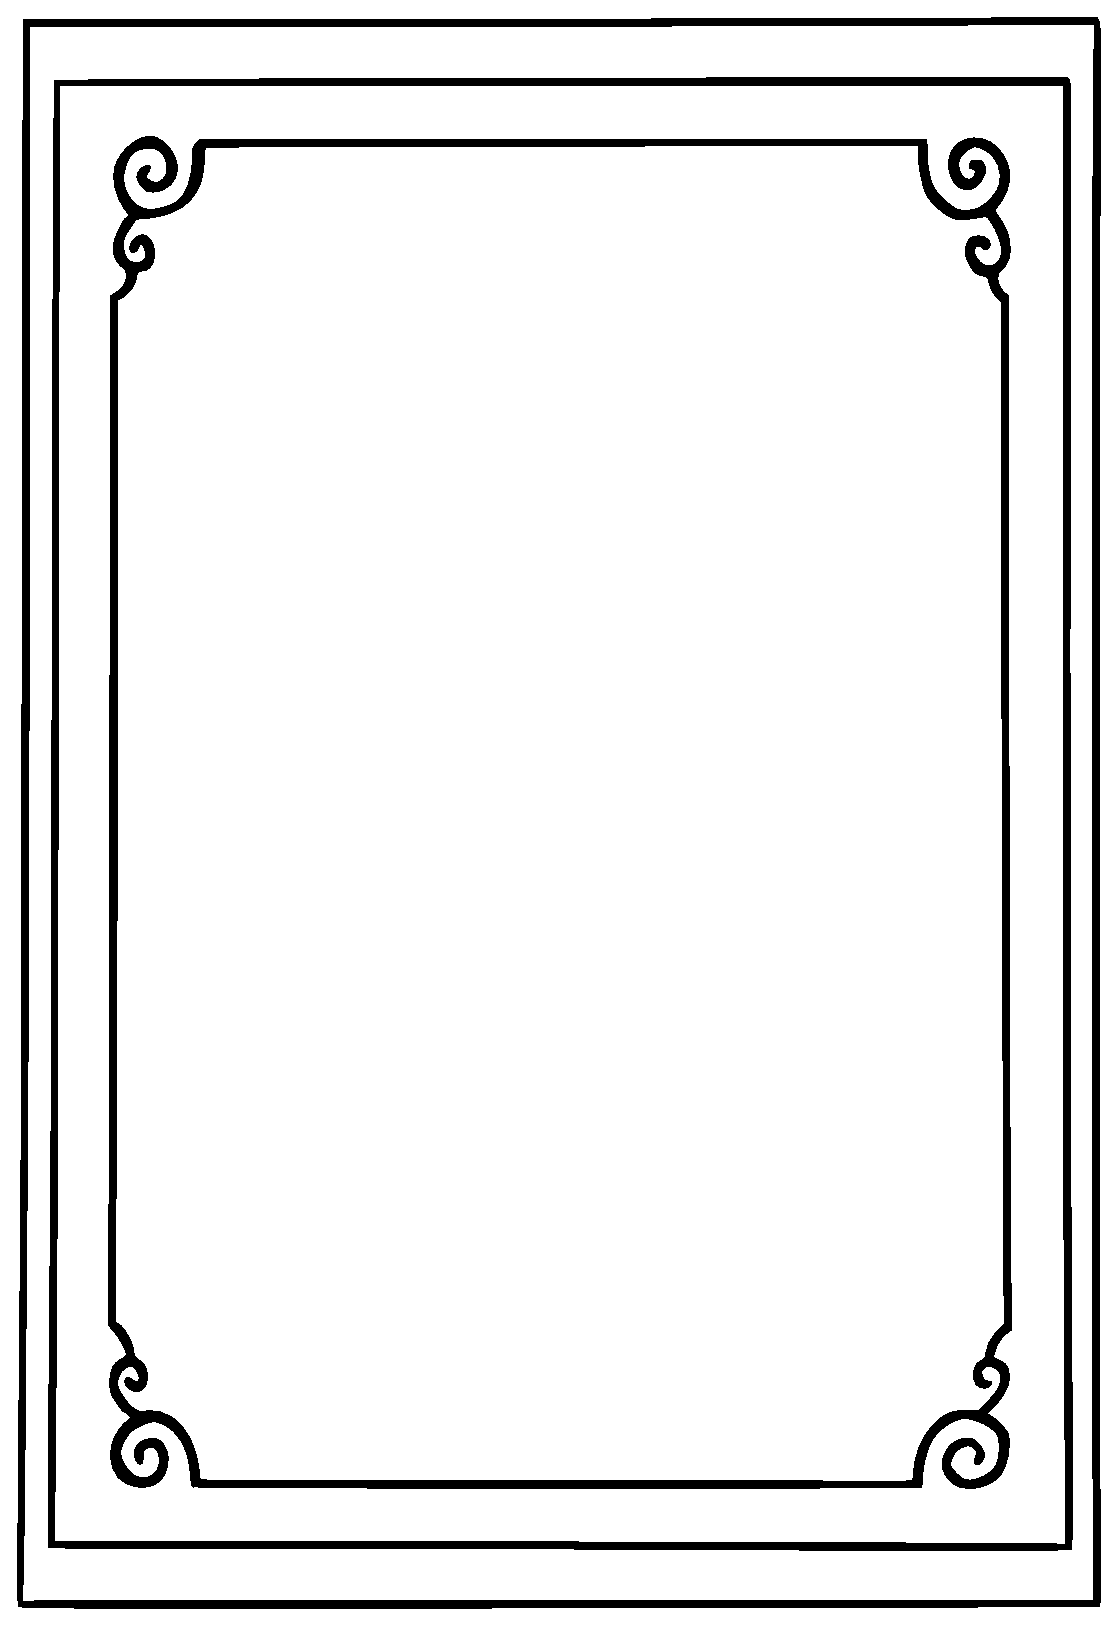
\includegraphics[width=0.96\textwidth]{cornice}
}
\clearpage

%% -- PAGINA DI RIEMPIMENTO
Antani
\end{document}

